% Options for packages loaded elsewhere
\PassOptionsToPackage{unicode}{hyperref}
\PassOptionsToPackage{hyphens}{url}
%
\documentclass[
]{article}
\usepackage{amsmath,amssymb}
\usepackage{iftex}
\ifPDFTeX
  \usepackage[T1]{fontenc}
  \usepackage[utf8]{inputenc}
  \usepackage{textcomp} % provide euro and other symbols
\else % if luatex or xetex
  \usepackage{unicode-math} % this also loads fontspec
  \defaultfontfeatures{Scale=MatchLowercase}
  \defaultfontfeatures[\rmfamily]{Ligatures=TeX,Scale=1}
\fi
\usepackage{lmodern}
\ifPDFTeX\else
  % xetex/luatex font selection
\fi
% Use upquote if available, for straight quotes in verbatim environments
\IfFileExists{upquote.sty}{\usepackage{upquote}}{}
\IfFileExists{microtype.sty}{% use microtype if available
  \usepackage[]{microtype}
  \UseMicrotypeSet[protrusion]{basicmath} % disable protrusion for tt fonts
}{}
\makeatletter
\@ifundefined{KOMAClassName}{% if non-KOMA class
  \IfFileExists{parskip.sty}{%
    \usepackage{parskip}
  }{% else
    \setlength{\parindent}{0pt}
    \setlength{\parskip}{6pt plus 2pt minus 1pt}}
}{% if KOMA class
  \KOMAoptions{parskip=half}}
\makeatother
\usepackage{xcolor}
\usepackage[margin=1in]{geometry}
\usepackage{color}
\usepackage{fancyvrb}
\newcommand{\VerbBar}{|}
\newcommand{\VERB}{\Verb[commandchars=\\\{\}]}
\DefineVerbatimEnvironment{Highlighting}{Verbatim}{commandchars=\\\{\}}
% Add ',fontsize=\small' for more characters per line
\usepackage{framed}
\definecolor{shadecolor}{RGB}{248,248,248}
\newenvironment{Shaded}{\begin{snugshade}}{\end{snugshade}}
\newcommand{\AlertTok}[1]{\textcolor[rgb]{0.94,0.16,0.16}{#1}}
\newcommand{\AnnotationTok}[1]{\textcolor[rgb]{0.56,0.35,0.01}{\textbf{\textit{#1}}}}
\newcommand{\AttributeTok}[1]{\textcolor[rgb]{0.13,0.29,0.53}{#1}}
\newcommand{\BaseNTok}[1]{\textcolor[rgb]{0.00,0.00,0.81}{#1}}
\newcommand{\BuiltInTok}[1]{#1}
\newcommand{\CharTok}[1]{\textcolor[rgb]{0.31,0.60,0.02}{#1}}
\newcommand{\CommentTok}[1]{\textcolor[rgb]{0.56,0.35,0.01}{\textit{#1}}}
\newcommand{\CommentVarTok}[1]{\textcolor[rgb]{0.56,0.35,0.01}{\textbf{\textit{#1}}}}
\newcommand{\ConstantTok}[1]{\textcolor[rgb]{0.56,0.35,0.01}{#1}}
\newcommand{\ControlFlowTok}[1]{\textcolor[rgb]{0.13,0.29,0.53}{\textbf{#1}}}
\newcommand{\DataTypeTok}[1]{\textcolor[rgb]{0.13,0.29,0.53}{#1}}
\newcommand{\DecValTok}[1]{\textcolor[rgb]{0.00,0.00,0.81}{#1}}
\newcommand{\DocumentationTok}[1]{\textcolor[rgb]{0.56,0.35,0.01}{\textbf{\textit{#1}}}}
\newcommand{\ErrorTok}[1]{\textcolor[rgb]{0.64,0.00,0.00}{\textbf{#1}}}
\newcommand{\ExtensionTok}[1]{#1}
\newcommand{\FloatTok}[1]{\textcolor[rgb]{0.00,0.00,0.81}{#1}}
\newcommand{\FunctionTok}[1]{\textcolor[rgb]{0.13,0.29,0.53}{\textbf{#1}}}
\newcommand{\ImportTok}[1]{#1}
\newcommand{\InformationTok}[1]{\textcolor[rgb]{0.56,0.35,0.01}{\textbf{\textit{#1}}}}
\newcommand{\KeywordTok}[1]{\textcolor[rgb]{0.13,0.29,0.53}{\textbf{#1}}}
\newcommand{\NormalTok}[1]{#1}
\newcommand{\OperatorTok}[1]{\textcolor[rgb]{0.81,0.36,0.00}{\textbf{#1}}}
\newcommand{\OtherTok}[1]{\textcolor[rgb]{0.56,0.35,0.01}{#1}}
\newcommand{\PreprocessorTok}[1]{\textcolor[rgb]{0.56,0.35,0.01}{\textit{#1}}}
\newcommand{\RegionMarkerTok}[1]{#1}
\newcommand{\SpecialCharTok}[1]{\textcolor[rgb]{0.81,0.36,0.00}{\textbf{#1}}}
\newcommand{\SpecialStringTok}[1]{\textcolor[rgb]{0.31,0.60,0.02}{#1}}
\newcommand{\StringTok}[1]{\textcolor[rgb]{0.31,0.60,0.02}{#1}}
\newcommand{\VariableTok}[1]{\textcolor[rgb]{0.00,0.00,0.00}{#1}}
\newcommand{\VerbatimStringTok}[1]{\textcolor[rgb]{0.31,0.60,0.02}{#1}}
\newcommand{\WarningTok}[1]{\textcolor[rgb]{0.56,0.35,0.01}{\textbf{\textit{#1}}}}
\usepackage{graphicx}
\makeatletter
\def\maxwidth{\ifdim\Gin@nat@width>\linewidth\linewidth\else\Gin@nat@width\fi}
\def\maxheight{\ifdim\Gin@nat@height>\textheight\textheight\else\Gin@nat@height\fi}
\makeatother
% Scale images if necessary, so that they will not overflow the page
% margins by default, and it is still possible to overwrite the defaults
% using explicit options in \includegraphics[width, height, ...]{}
\setkeys{Gin}{width=\maxwidth,height=\maxheight,keepaspectratio}
% Set default figure placement to htbp
\makeatletter
\def\fps@figure{htbp}
\makeatother
\setlength{\emergencystretch}{3em} % prevent overfull lines
\providecommand{\tightlist}{%
  \setlength{\itemsep}{0pt}\setlength{\parskip}{0pt}}
\setcounter{secnumdepth}{-\maxdimen} % remove section numbering
\ifLuaTeX
  \usepackage{selnolig}  % disable illegal ligatures
\fi
\IfFileExists{bookmark.sty}{\usepackage{bookmark}}{\usepackage{hyperref}}
\IfFileExists{xurl.sty}{\usepackage{xurl}}{} % add URL line breaks if available
\urlstyle{same}
\hypersetup{
  pdftitle={Primer parcial},
  pdfauthor={Daniel Gonzalez},
  hidelinks,
  pdfcreator={LaTeX via pandoc}}

\title{Primer parcial}
\author{Daniel Gonzalez}
\date{2023-08-29}

\begin{document}
\maketitle

\hypertarget{problema-1}{%
\subsubsection{Problema 1}\label{problema-1}}

{[}1.{]} En Colombia, durante un período histórico, se creía que la
distribución de grupos sanguíneos era la siguiente: tipo A, 32\%; tipo
B, 24\%; tipo AB, 5\%; y tipo O, 39\%. Se estimaba que en ese tiempo, el
3\% de las personas pertenecientes al tipo O fue clasificado como del
tipo A; el 90\% de los del tipo A fue correctamente clasificado; el 5\%
de los del tipo B se clasificó como del tipo A, y el 8\% de los del tipo
AB fue clasificado incorrectamente como del tipo A. Un soldado herido
fue llevado a la enfermería y se le clasificó como del tipo A. ¿Cuál es
la probabilidad de que tal grupo sanguíneo sea ciertamente el suyo?

\hypertarget{solucion}{%
\subsubsection{\texorpdfstring{\textbf{Solucion}}{Solucion}}\label{solucion}}

Utilizaremos el teorema de Bayes para calcular la probabilidad
condicional:

\[\begin{align*}
        P(\text{Tipo A}|\text{Clasificado como Tipo A}) &= \frac{P(\text{Clasificado como Tipo A}|\text{Tipo A}) \cdot P(\text{Tipo A})}{P(\text{Clasificado como Tipo A})} \\
        &= \frac{0.90 \cdot 0.32}{P(\text{Clasificado como Tipo A})}
    \end{align*}
\]

Para calcular \(P(\text{Clasificado como Tipo A})\), utilizamos la ley
de probabilidad total:

\[  
\begin{align*}
        P(\text{Clasificado como Tipo A}) &= P(\text{Clasificado como Tipo A}|\text{Tipo A}) \cdot P(\text{Tipo A}) \\
        &+ P(\text{Clasificado como Tipo A}|\text{Tipo B}) \cdot P(\text{Tipo B}) \\
        &+ P(\text{Clasificado como Tipo A}|\text{Tipo AB}) \cdot P(\text{Tipo AB}) \\
        &+ P(\text{Clasificado como Tipo A}|\text{Tipo O}) \cdot P(\text{Tipo O}) \\
        &= (0.90 \cdot 0.32) + (0.05 \cdot 0.24) + (0.08 \cdot 0.05) + (0.03 \cdot 0.39)
\end{align*}
\]

Finalmente, podemos calcular la probabilidad:

\[
\begin{align*}
        P(\text{Tipo A}|\text{Clasificado como Tipo A}) &= \frac{0.90 \cdot 0.32}{(0.90 \cdot 0.32) + (0.05 \cdot 0.24) + (0.08 \cdot 0.05) + (0.03 \cdot 0.39)} \\
        &\approx \frac{0.288}{0.2893} \\
        &\approx 0.9965
    \end{align*}
\]

Por lo tanto, la probabilidad de que el grupo sanguíneo del soldado sea
ciertamente Tipo A es aproximadamente del 99.65\%.

\hypertarget{problema-2}{%
\subsubsection{Problema 2}\label{problema-2}}

{[}2.{]} Elabore un gráfico para representar adecuadamente la siguiente
información:

{[}a.{]} Durante 5 meses se construyen 134 kilómetros de carretera en la
siguiente forma: En el primer mes, 3.60\% del total del proyecto; en el
segundo mes un 7.60\% del total; en el tercer mes, el 15.3\% del total;
en el cuarto mes 24.5\% del total y en último mes, el 49\% restante.

\begin{Shaded}
\begin{Highlighting}[]
\CommentTok{\# Instala y carga la biblioteca ggplot2 si aún no está instalada}
\ControlFlowTok{if}\NormalTok{ (}\SpecialCharTok{!}\FunctionTok{requireNamespace}\NormalTok{(}\StringTok{"ggplot2"}\NormalTok{, }\AttributeTok{quietly =} \ConstantTok{TRUE}\NormalTok{)) \{}
  \FunctionTok{install.packages}\NormalTok{(}\StringTok{"ggplot2"}\NormalTok{)}
\NormalTok{\}}
\FunctionTok{library}\NormalTok{(ggplot2)}

\CommentTok{\# Datos}
\NormalTok{meses }\OtherTok{\textless{}{-}} \FunctionTok{c}\NormalTok{(}\StringTok{"Mes 1"}\NormalTok{, }\StringTok{"Mes 2"}\NormalTok{, }\StringTok{"Mes 3"}\NormalTok{, }\StringTok{"Mes 4"}\NormalTok{, }\StringTok{"Mes 5"}\NormalTok{)}
\NormalTok{porcentaje\_construido }\OtherTok{\textless{}{-}} \FunctionTok{c}\NormalTok{(}\FloatTok{3.60}\NormalTok{, }\FloatTok{7.60}\NormalTok{, }\FloatTok{15.3}\NormalTok{, }\FloatTok{24.5}\NormalTok{, }\FloatTok{49.0}\NormalTok{)}
\NormalTok{total\_proyecto }\OtherTok{\textless{}{-}} \DecValTok{134}  \CommentTok{\# Total de kilómetros del proyecto}

\CommentTok{\# Calcula los kilómetros construidos en cada mes}
\NormalTok{kilometros\_construidos }\OtherTok{\textless{}{-}}\NormalTok{ porcentaje\_construido }\SpecialCharTok{*}\NormalTok{ total\_proyecto }\SpecialCharTok{/} \DecValTok{100}

\CommentTok{\# Crea un marco de datos con los datos}
\NormalTok{data }\OtherTok{\textless{}{-}} \FunctionTok{data.frame}\NormalTok{(}\AttributeTok{Mes =}\NormalTok{ meses, }\AttributeTok{Kilometros\_Construidos =}\NormalTok{ kilometros\_construidos)}

\CommentTok{\# Crea el gráfico de líneas}
\FunctionTok{ggplot}\NormalTok{(data, }\FunctionTok{aes}\NormalTok{(}\AttributeTok{x =}\NormalTok{ Mes, }\AttributeTok{y =}\NormalTok{ Kilometros\_Construidos, }\AttributeTok{group =} \DecValTok{1}\NormalTok{)) }\SpecialCharTok{+}
  \FunctionTok{geom\_line}\NormalTok{() }\SpecialCharTok{+}
  \FunctionTok{geom\_point}\NormalTok{() }\SpecialCharTok{+}
  \FunctionTok{labs}\NormalTok{(}
    \AttributeTok{title =} \StringTok{"Construcción de la carretera por mes"}\NormalTok{,}
    \AttributeTok{x =} \StringTok{"Mes"}\NormalTok{,}
    \AttributeTok{y =} \StringTok{"Kilómetros Construidos"}
\NormalTok{  ) }\SpecialCharTok{+}
  \FunctionTok{theme\_minimal}\NormalTok{()}
\end{Highlighting}
\end{Shaded}

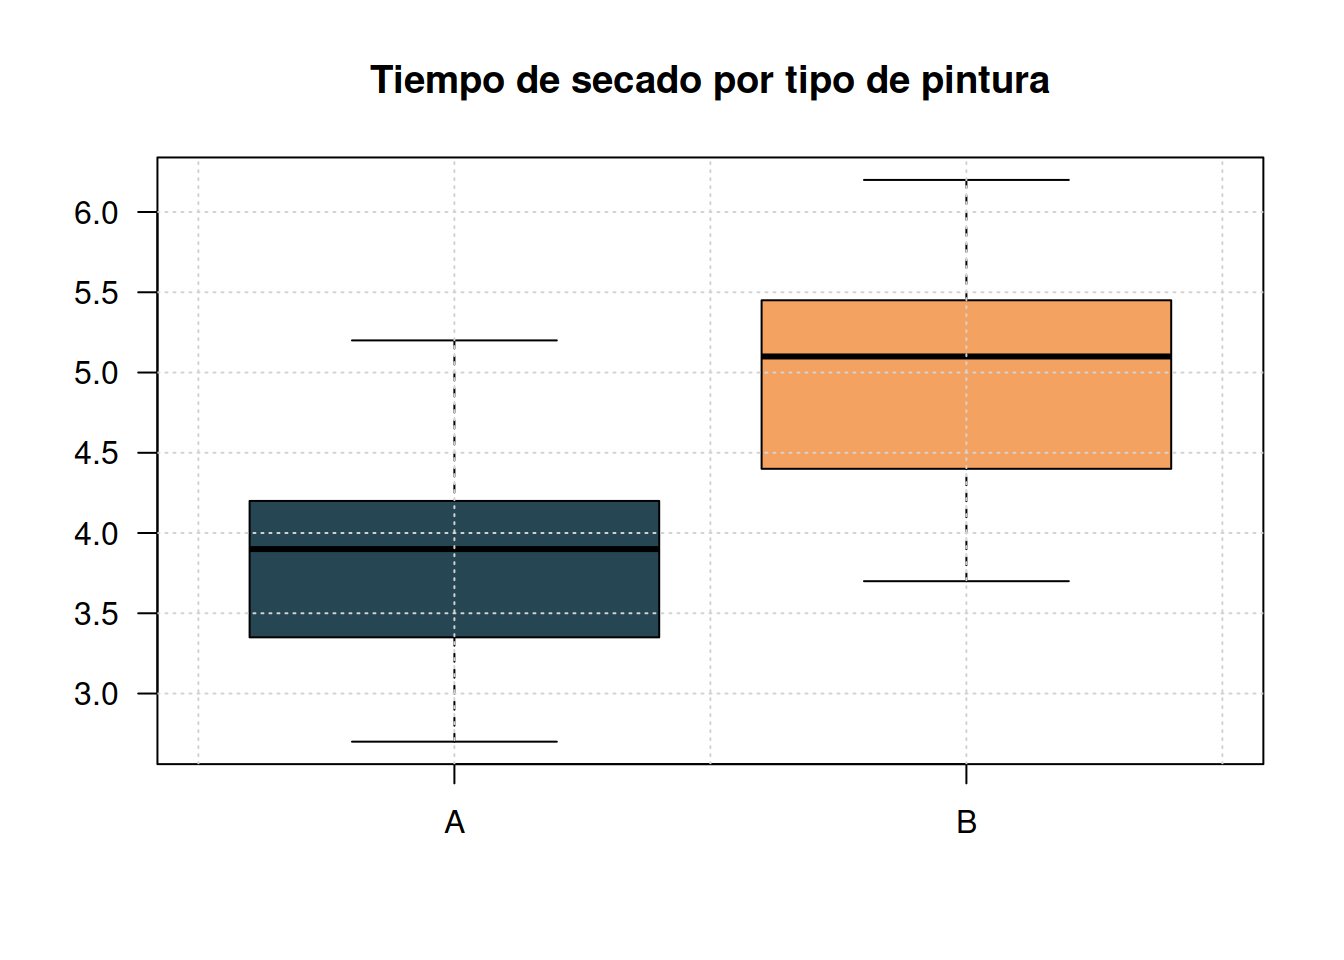
\includegraphics{primer_parcial20232_files/figure-latex/unnamed-chunk-1-1.pdf}

{[}b.{]} El grupo de Estadística a cargo de un profesor está conformado
por : 9 estudiantes de Ingeniería Electrónica, 6 de Ingeniería de
Sistemas, 25 de Ingeniería Civil, 19 de Negocios Internacionales 8 de
Biología y 3 de Ingeniería Mecánica. De los que estudian Ingeniería
Electrónica 6 son hombres, de los matriculados en Ingeniería de Sistemas
2 son mujeres, de los que estudian Ingeniería Civil 18 son hombres, de
los que estudian Negocios internacionales 16 son mujeres, de los que
estudian Biología 5 son mujeres y finalmente de los que estudian
Ingeniería Mecánica 2 son hombre.

\begin{Shaded}
\begin{Highlighting}[]
\CommentTok{\# Definir la matriz de datos}
\NormalTok{tabla }\OtherTok{\textless{}{-}} \FunctionTok{matrix}\NormalTok{(}\FunctionTok{c}\NormalTok{(}\DecValTok{6}\NormalTok{, }\DecValTok{2}\NormalTok{, }\DecValTok{18}\NormalTok{, }\DecValTok{2}\NormalTok{, }\DecValTok{2}\NormalTok{, }\DecValTok{2}\NormalTok{, }\DecValTok{3}\NormalTok{, }\DecValTok{4}\NormalTok{, }\DecValTok{7}\NormalTok{, }\DecValTok{16}\NormalTok{, }\DecValTok{3}\NormalTok{, }\DecValTok{1}\NormalTok{),}
                \AttributeTok{nrow =} \DecValTok{2}\NormalTok{, }\AttributeTok{byrow =} \ConstantTok{TRUE}\NormalTok{)}

\CommentTok{\# Definir los nombres de fila y columna}
\FunctionTok{rownames}\NormalTok{(tabla) }\OtherTok{\textless{}{-}} \FunctionTok{c}\NormalTok{(}\StringTok{"Hombres"}\NormalTok{, }\StringTok{"Mujeres"}\NormalTok{)}
\FunctionTok{colnames}\NormalTok{(tabla) }\OtherTok{\textless{}{-}} \FunctionTok{c}\NormalTok{(}\StringTok{"Electrónica"}\NormalTok{, }\StringTok{"Sistemas"}\NormalTok{, }\StringTok{"Civil"}\NormalTok{, }\StringTok{"Internacional"}\NormalTok{, }\StringTok{"Biología"}\NormalTok{, }\StringTok{"Mecánica"}\NormalTok{)}

\CommentTok{\# Colores para hombres y mujeres}
\NormalTok{colores }\OtherTok{\textless{}{-}} \FunctionTok{c}\NormalTok{(}\StringTok{"blue"}\NormalTok{, }\StringTok{"pink"}\NormalTok{)}

\CommentTok{\# Crear el gráfico de barras con colores y leyendas}
\FunctionTok{barplot}\NormalTok{(tabla, }\AttributeTok{beside =} \ConstantTok{TRUE}\NormalTok{, }\AttributeTok{col =}\NormalTok{ colores,}
        \AttributeTok{legend.text =} \FunctionTok{rownames}\NormalTok{(tabla), }\AttributeTok{args.legend =} \FunctionTok{list}\NormalTok{(}\AttributeTok{x =} \StringTok{"topright"}\NormalTok{, }\AttributeTok{bty =} \StringTok{"n"}\NormalTok{, }\AttributeTok{ncol =} \DecValTok{1}\NormalTok{))}
\end{Highlighting}
\end{Shaded}

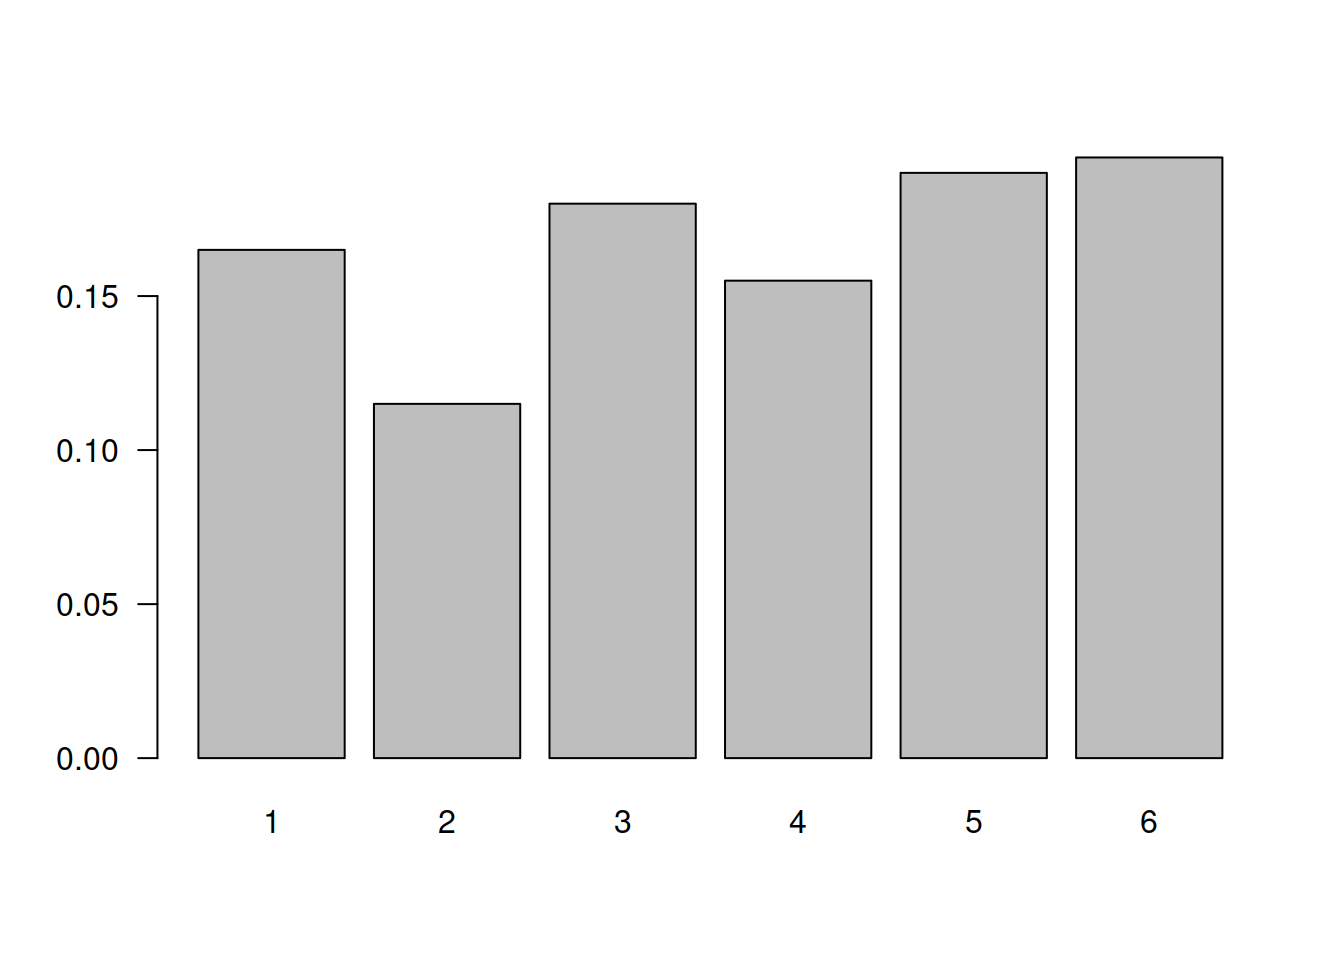
\includegraphics{primer_parcial20232_files/figure-latex/unnamed-chunk-2-1.pdf}

{[}c.{]} Una consulta en tiendas en linea para memorias USB 128GB arrojó
lo siguientes valores:

6\textbar0 3 4 7 8 8 8 7\textbar0 0 1 1 2 2 2 3 3 4 4 5 5 5 5 5 6 6 7 7
9 8\textbar0 3 3 4 5 6 7 8 8 9 9 9\textbar1

\begin{Shaded}
\begin{Highlighting}[]
\CommentTok{\# Datos a partir del diagrama de tallos y hojas}
\NormalTok{datos }\OtherTok{\textless{}{-}} \FunctionTok{c}\NormalTok{(}\DecValTok{60}\NormalTok{, }\DecValTok{63}\NormalTok{, }\DecValTok{64}\NormalTok{, }\DecValTok{67}\NormalTok{, }\DecValTok{68}\NormalTok{, }\DecValTok{68}\NormalTok{, }\DecValTok{68}\NormalTok{, }\DecValTok{70}\NormalTok{, }\DecValTok{70}\NormalTok{, }\DecValTok{71}\NormalTok{, }\DecValTok{71}\NormalTok{, }\DecValTok{72}\NormalTok{, }\DecValTok{72}\NormalTok{, }\DecValTok{72}\NormalTok{, }\DecValTok{72}\NormalTok{, }\DecValTok{72}\NormalTok{, }\DecValTok{73}\NormalTok{, }\DecValTok{73}\NormalTok{, }\DecValTok{74}\NormalTok{, }\DecValTok{74}\NormalTok{, }\DecValTok{75}\NormalTok{, }\DecValTok{75}\NormalTok{, }\DecValTok{75}\NormalTok{, }\DecValTok{75}\NormalTok{, }\DecValTok{75}\NormalTok{, }\DecValTok{80}\NormalTok{, }\DecValTok{83}\NormalTok{, }\DecValTok{83}\NormalTok{, }\DecValTok{84}\NormalTok{, }\DecValTok{85}\NormalTok{, }\DecValTok{86}\NormalTok{, }\DecValTok{87}\NormalTok{, }\DecValTok{88}\NormalTok{, }\DecValTok{88}\NormalTok{, }\DecValTok{89}\NormalTok{, }\DecValTok{89}\NormalTok{, }\DecValTok{90}\NormalTok{, }\DecValTok{91}\NormalTok{)}

\CommentTok{\# Crear el histograma}
\FunctionTok{boxplot}\NormalTok{(datos, }\AttributeTok{main =} \StringTok{"Histograma de Datos"}\NormalTok{, }\AttributeTok{xlab =} \StringTok{"Valores"}\NormalTok{, }\AttributeTok{ylab =} \StringTok{"Frecuencia"}\NormalTok{, }\AttributeTok{col =} \StringTok{"blue"}\NormalTok{, }\AttributeTok{border =} \StringTok{"black"}\NormalTok{, }\AttributeTok{breaks =} \DecValTok{10}\NormalTok{)}
\end{Highlighting}
\end{Shaded}

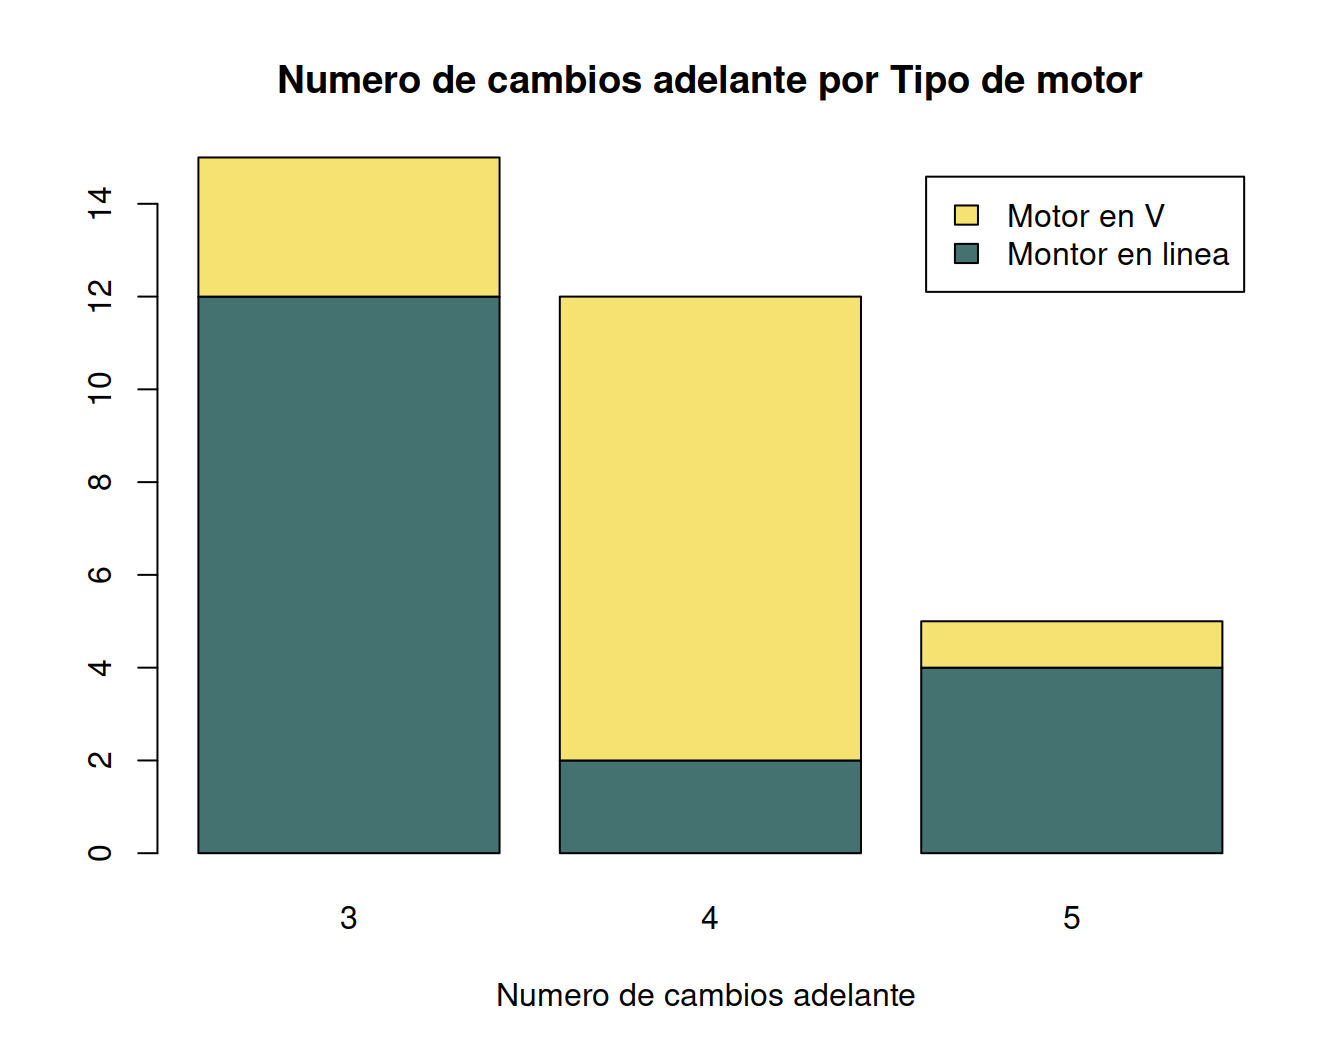
\includegraphics{primer_parcial20232_files/figure-latex/unnamed-chunk-3-1.pdf}

{[}d.{]} La clasificación de los empleados de una empresa por cargo es
la siguiente: un Administradores, tres Ingenieros, treinta operarios,
ocho celadores, dos contadores, tres secretarias, cinco supervisores,
treinta y seis vendedores.

\begin{Shaded}
\begin{Highlighting}[]
\CommentTok{\# Definir los datos}
\NormalTok{cargos }\OtherTok{\textless{}{-}} \FunctionTok{c}\NormalTok{(}\StringTok{"Administradores"}\NormalTok{, }\StringTok{"Ingenieros"}\NormalTok{, }\StringTok{"Operarios"}\NormalTok{, }\StringTok{"Celadores"}\NormalTok{, }\StringTok{"Contadores"}\NormalTok{, }\StringTok{"Secretarias"}\NormalTok{, }\StringTok{"Supervisores"}\NormalTok{, }\StringTok{"Vendedores"}\NormalTok{)}
\NormalTok{cantidad }\OtherTok{\textless{}{-}} \FunctionTok{c}\NormalTok{(}\DecValTok{1}\NormalTok{, }\DecValTok{3}\NormalTok{, }\DecValTok{30}\NormalTok{, }\DecValTok{8}\NormalTok{, }\DecValTok{2}\NormalTok{, }\DecValTok{3}\NormalTok{, }\DecValTok{5}\NormalTok{, }\DecValTok{36}\NormalTok{)}

\CommentTok{\# Calcular los porcentajes}
\NormalTok{porcentajes }\OtherTok{\textless{}{-}} \FunctionTok{round}\NormalTok{(cantidad }\SpecialCharTok{/} \FunctionTok{sum}\NormalTok{(cantidad) }\SpecialCharTok{*} \DecValTok{100}\NormalTok{, }\DecValTok{1}\NormalTok{)}

\CommentTok{\# Crear el gráfico de torta con porcentajes}
\FunctionTok{pie}\NormalTok{(cantidad, }\AttributeTok{labels =} \FunctionTok{paste}\NormalTok{(cargos, }\StringTok{"("}\NormalTok{, porcentajes, }\StringTok{"\%)"}\NormalTok{), }\AttributeTok{col =} \FunctionTok{rainbow}\NormalTok{(}\FunctionTok{length}\NormalTok{(cargos)), }\AttributeTok{main =} \StringTok{"Clasificación de Empleados por Cargo"}\NormalTok{)}
\end{Highlighting}
\end{Shaded}

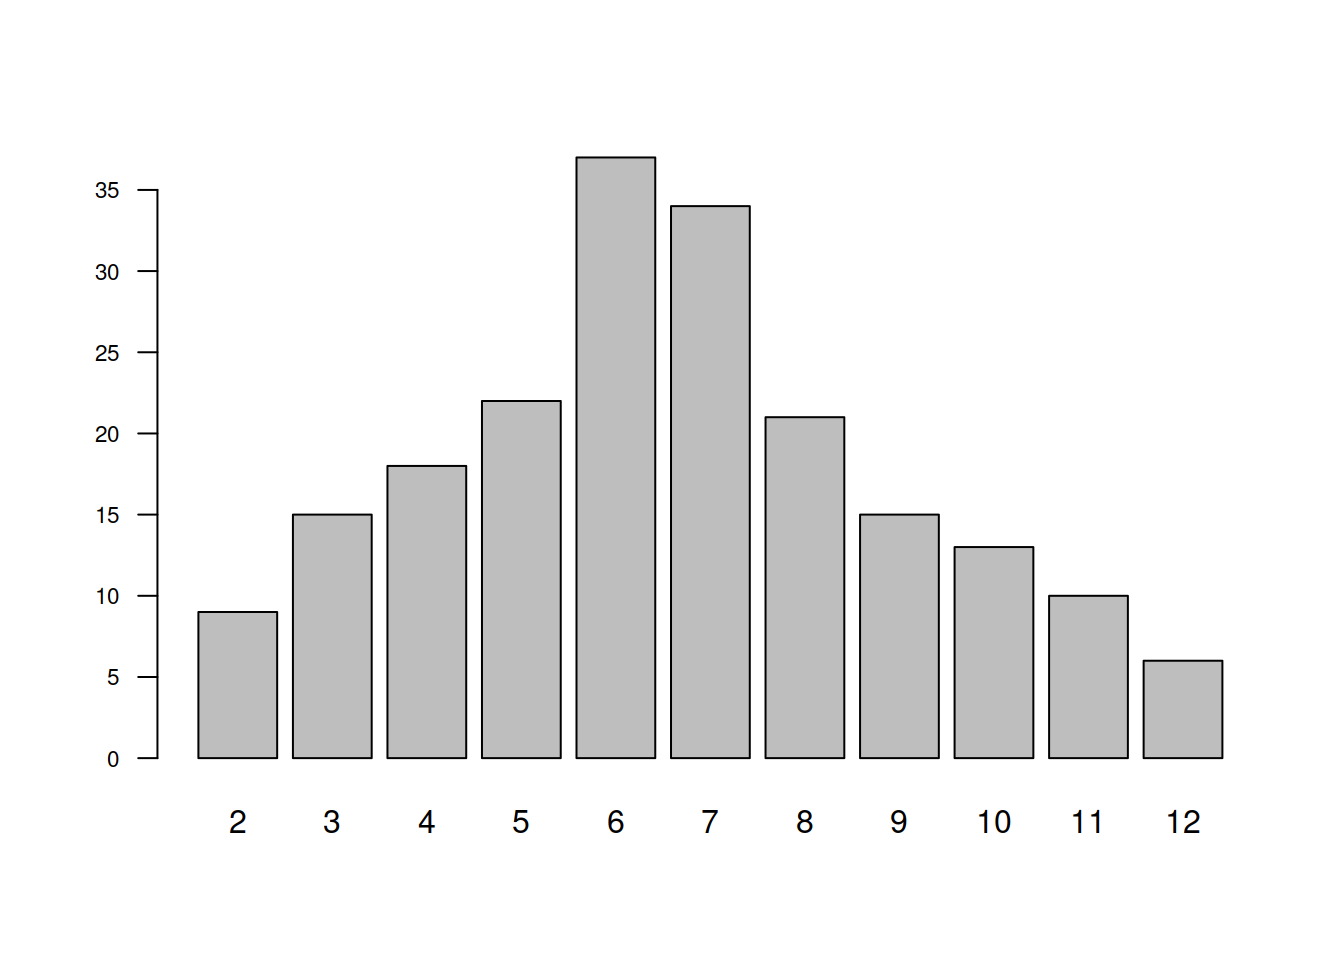
\includegraphics{primer_parcial20232_files/figure-latex/unnamed-chunk-4-1.pdf}

\hypertarget{problema-3}{%
\subsubsection{Problema 3}\label{problema-3}}

{[}3.{]} Para analizar la rapidez con que una máquina etiqueta las
botellas en una compañía de jugos, se decide hacer seguimiento al número
de botellas etiquetadas por día. A partir de los resultados procesados
en R presente un análisis estadístico para el número de botellas
etiquetadas por día

\begin{Shaded}
\begin{Highlighting}[]
\CommentTok{\# }
\CommentTok{\# summarytools::descr(x)  }
\CommentTok{\# }
\CommentTok{\# Mean      7457.79}
\CommentTok{\# Std.Dev    826.51}
\CommentTok{\# Min       5944.00}
\CommentTok{\# Q1        6839.50}
\CommentTok{\# Median    7455.00}
\CommentTok{\# Q3        8117.00}
\CommentTok{\# Max       9121.00}
\CommentTok{\# MAD        956.28}
\CommentTok{\# IQR       1269.25}
\CommentTok{\# CV           0.11}
\CommentTok{\# Skewness     0.11}
\CommentTok{\# SE.Skewness  0.34}
\CommentTok{\# Kurtosis    {-}1.01}
\CommentTok{\# N.Valid      8.00}
\CommentTok{\# Pct.Valid  100.00}
\end{Highlighting}
\end{Shaded}

Elabore una descripción de la información obtenida

\hypertarget{solucion-1}{%
\subsubsection{\texorpdfstring{\textbf{Solucion}}{Solucion}}\label{solucion-1}}

Basándonos en los estadísticos proporcionados y considerando la
asimetría ligeramente positiva de 0.11, podemos decir que la
distribución del número de botellas etiquetadas por día en la compañía
de jugos parece tener una tendencia hacia la derecha. Esto sugiere que
la mayoría de los días, el número de botellas etiquetadas es cercano o
superior a la media de 7,457.79 botellas. La medida de centro que mejor
representa la distribución en este caso es la mediana, que es de
7,455.00 botellas por día. El coeficiente de variación del 11\% indica
una moderada variabilidad en relación con la media. En conjunto, estos
datos sugieren que, en general, la producción de etiquetado tiende a ser
consistente, pero puede haber días con un mayor número de botellas
etiquetadas que se desvían significativamente de la media, lo que
resulta en una ligera asimetría hacia la derecha en la distribución.

\hypertarget{problema-1-1}{%
\subsubsection{Problema 1}\label{problema-1-1}}

{[}1.{]} En un estudio sobre preferencias de alimentos en una escuela,
se encontró que el 60\% de los estudiantes prefieren la pizza, el 25\%
prefieren hamburguesas, el 10\% prefiere tacos y el 5\% tiene otras
preferencias. Además, se sabe que el 80\% de los que prefieren pizza
fueron identificados correctamente, el 70\% de los que prefieren
hamburguesas fueron identificados correctamente, el 50\% de los que
prefieren tacos fueron identificados correctamente, y el 40\% de los que
tienen otras preferencias fueron clasificados incorrectamente. Un
estudiante es seleccionado al azar y se le identifica como alguien que
prefiere pizza. ¿Cuál es la probabilidad de que en realidad prefiera
pizza?

\hypertarget{solucion-2}{%
\subsubsection{\texorpdfstring{\textbf{Solucion}}{Solucion}}\label{solucion-2}}

Para calcular la probabilidad de que un estudiante que fue identificado
como alguien que prefiere pizza realmente prefiera pizza, podemos
utilizar el teorema de Bayes. Denotemos los siguientes eventos:

\begin{itemize}
\tightlist
\item
  A: El estudiante realmente prefiere pizza.
\item
  B: El estudiante fue identificado como alguien que prefiere pizza.
\end{itemize}

Tenemos la siguiente información:

\begin{itemize}
\tightlist
\item
  P(A) = Probabilidad de que un estudiante prefiera pizza = 60\% = 0.60.
\item
  P(B\textbar A) = Probabilidad de que un estudiante sea identificado
  correctamente si prefiere pizza = 80\% = 0.80.
\item
  P(B\textbar¬A) = Probabilidad de que un estudiante sea identificado
  incorrectamente si no prefiere pizza = 40\% = 0.40.
\end{itemize}

Queremos encontrar P(A\textbar B), es decir, la probabilidad de que un
estudiante realmente prefiera pizza dado que fue identificado como
alguien que prefiere pizza.

Utilizando el teorema de Bayes:

\[P(A|B) = \frac{P(A) \cdot P(B|A)}{P(A) \cdot P(B|A) + P(¬A) \cdot P(B|¬A)}\]

Sustituyendo los valores conocidos:

\[P(A|B) = \frac{0.60 \cdot 0.80}{0.60 \cdot 0.80 + (1 - 0.60) \cdot 0.40}\]

\[P(A|B) = \frac{0.48}{0.48 + 0.40 \cdot 0.40}\]

\[P(A|B) = \frac{0.48}{0.48 + 0.16}\]

\[P(A|B) = \frac{0.48}{0.64}\]

\[P(A|B) = 0.75\]

Por lo tanto, la probabilidad de que un estudiante que fue identificado
como alguien que prefiere pizza realmente prefiera pizza es del 75\%.

\hypertarget{problema-1-2}{%
\subsubsection{Problema 1}\label{problema-1-2}}

{[}1.{]} En el colegio Anglo-Frances se imparten sólo los idiomas inglés
y francés. El 80\% de los alumnos estudian inglés y el resto francés. El
30\% de los alumnos que cursan de inglés son socio del club musical del
colegio, mientras de los que estudian francés son socio de dicho club el
40\%. Si el director del colegio elige un alumno de manera aleatoria,
¿qué tan probable es que dicho alumno pertenezca al club de musical? .
Por otra parte el psicólogo del colegio afirma que estudiar inglés es un
evento independiente de estudiar francés. ¿usted que opina respecto a
esta afirmación? (justifique su respuesta)

\hypertarget{solucion-3}{%
\subsubsection{\texorpdfstring{\textbf{Solucion}}{Solucion}}\label{solucion-3}}

Para calcular la probabilidad de que un alumno elegido al azar
pertenezca al club musical, primero necesitamos calcular la probabilidad
condicional basada en si el estudiante estudia inglés o francés. Luego,
evaluaremos la independencia entre estudiar inglés y francés.

Denotemos los siguientes eventos:

\begin{itemize}
\tightlist
\item
  I: Estudiar inglés.
\item
  F: Estudiar francés.
\item
  M: Ser socio del club musical.
\end{itemize}

Tenemos la siguiente información:

\begin{itemize}
\tightlist
\item
  P(I) = Probabilidad de estudiar inglés = 80\% = 0.80.
\item
  P(F) = Probabilidad de estudiar francés = 20\% = 0.20.
\item
  P(M\textbar I) = Probabilidad de ser socio del club musical dado que
  estudia inglés = 30\% = 0.30.
\item
  P(M\textbar F) = Probabilidad de ser socio del club musical dado que
  estudia francés = 40\% = 0.40.
\end{itemize}

Primero, calculamos la probabilidad de que un estudiante elegido al azar
sea socio del club musical:

\[P(M) = P(M|I) \cdot P(I) + P(M|F) \cdot P(F)\]
\[P(M) = (0.30 \cdot 0.80) + (0.40 \cdot 0.20)\] \[P(M) = 0.24 + 0.08\]
\[P(M) = 0.32\]

Por lo tanto, la probabilidad de que un alumno elegido al azar
pertenezca al club musical es del 32\%.

Respecto a la afirmación del psicólogo de que estudiar inglés es un
evento independiente de estudiar francés, podemos evaluar esto mediante
la definición de independencia de eventos:

Dos eventos son independientes si y solo si:

\[P(I ∩ F) = P(I) \cdot P(F)\]

Donde:

\begin{itemize}
\tightlist
\item
  \(P(I ∩ F)\) es la probabilidad de estudiar inglés y francés al mismo
  tiempo.
\item
  \(P(I)\) es la probabilidad de estudiar inglés.
\item
  \(P(F)\) es la probabilidad de estudiar francés.
\end{itemize}

Si los eventos son independientes, entonces esta ecuación debe ser
cierta. Si no es cierta, los eventos no son independientes.

En este caso:

\[P(I) = 0.80\] \[P(F) = 0.20\]

Sin embargo, no tenemos información sobre \(P(I ∩ F)\), es decir, no
sabemos la probabilidad de que un estudiante estudie ambos idiomas al
mismo tiempo. Por lo tanto, no podemos concluir si estudiar inglés y
francés son eventos independientes o no con la información
proporcionada. Necesitaríamos información adicional para determinar la
independencia de los eventos.

\hypertarget{problema-2-1}{%
\subsubsection{Problema 2}\label{problema-2-1}}

{[}2.{]} El director de la asociación de comerciantes de tomates del
Valle del Cauca estudia el comportamiento de las ventas diarias de los
últimos meses para una muestra de 60 nuevos microempresarios en la
región. Dos de las variables más importantes a tener en cuenta para el
estudio fueron: Ventas (meses Mayo y Junio) y el nivel tecnológico de la
empresa. La siguiente información corresponde a las ventas:

\begin{Shaded}
\begin{Highlighting}[]
\NormalTok{Julio }\OtherTok{=}\FunctionTok{c}\NormalTok{(}\FloatTok{14.3}\NormalTok{, }\FloatTok{14.4}\NormalTok{, }\FloatTok{11.1}\NormalTok{, }\FloatTok{11.2}\NormalTok{, }\FloatTok{11.4}\NormalTok{, }\FloatTok{11.4}\NormalTok{, }
         \FloatTok{11.4}\NormalTok{, }\FloatTok{11.4}\NormalTok{, }\FloatTok{10.0}\NormalTok{, }\FloatTok{10.5}\NormalTok{, }\FloatTok{10.5}\NormalTok{, }\FloatTok{10.6}\NormalTok{, }
         \FloatTok{10.7}\NormalTok{, }\FloatTok{12.1}\NormalTok{, }\FloatTok{12.3}\NormalTok{, }\FloatTok{12.4}\NormalTok{, }\FloatTok{12.8}\NormalTok{,  }\FloatTok{9.3}\NormalTok{,  }
         \FloatTok{9.2}\NormalTok{,  }\FloatTok{9.2}\NormalTok{, }\FloatTok{9.1}\NormalTok{,  }\FloatTok{8.4}\NormalTok{,  }\FloatTok{8.5}\NormalTok{,  }\FloatTok{7.2}\NormalTok{,  }
         \FloatTok{7.1}\NormalTok{,  }\FloatTok{6.2}\NormalTok{, }\FloatTok{13.7}\NormalTok{, }\FloatTok{13.8}\NormalTok{, }\FloatTok{15.0}\NormalTok{, }\FloatTok{10.0}\NormalTok{)}
    
\NormalTok{Agosto}\OtherTok{=}\FunctionTok{c}\NormalTok{(}\FloatTok{12.0}\NormalTok{, }\FloatTok{12.0}\NormalTok{, }\FloatTok{12.0}\NormalTok{, }\FloatTok{12.7}\NormalTok{, }\FloatTok{12.8}\NormalTok{, }\FloatTok{12.9}\NormalTok{, }
         \FloatTok{8.0}\NormalTok{, }\FloatTok{8.0}\NormalTok{, }\FloatTok{13.2}\NormalTok{, }\FloatTok{13.3}\NormalTok{, }\FloatTok{13.5}\NormalTok{, }\FloatTok{13.6}\NormalTok{, }
         \FloatTok{11.0}\NormalTok{, }\FloatTok{11.5}\NormalTok{, }\FloatTok{11.6}\NormalTok{, }\FloatTok{11.9}\NormalTok{, }\FloatTok{10.4}\NormalTok{, }\FloatTok{10.3}\NormalTok{, }
         \FloatTok{10.7}\NormalTok{,  }\FloatTok{9.0}\NormalTok{, }\FloatTok{9.2}\NormalTok{,  }\FloatTok{7.4}\NormalTok{,  }\FloatTok{7.7}\NormalTok{,  }\FloatTok{6.1}\NormalTok{,  }
         \FloatTok{5.9}\NormalTok{, }\FloatTok{14.3}\NormalTok{, }\FloatTok{14.2}\NormalTok{, }\FloatTok{14.8}\NormalTok{, }\FloatTok{15.1}\NormalTok{, }\FloatTok{15.2}\NormalTok{)}
\end{Highlighting}
\end{Shaded}

De acuerdo con la información anterior, responda \{\bf falso\} o
\{\bf verdadero\} a las siguientes premisas. En caso de ser falsa
justifique su respuesta.

\begin{enumerate}
\def\labelenumi{\alph{enumi}.}
\tightlist
\item
  La variable ventas mensuales se mide en escala de razón
\item
  Las ventas de 6.2 millones representan un dato atípico, para la
  información de Julio
\item
  Las ventas de Agosto son más homogeneas que las de Julio
\item
  La mediana de las ventas en el mes de Julio es de 11.15
\item
  La varianza para el mes de Julio es de 5.21
\item
  Aproximadamente el 68\% de las ventas de Julio están en el intervalo
  (8.7 ; 13.3)
\item
  Si el estado cobra un impuesto sobre las ventas del 16\%, el promedio
  del impuesto en Julio es de 1.75
\item
  El cuartil 1 (\(Q1\)) para las ventas de Agosto es 8.0
\item
  Las ventas de Julio muestran sesgo negativo
\end{enumerate}

\hypertarget{solucion-4}{%
\subsubsection{\texorpdfstring{\textbf{Solucion}}{Solucion}}\label{solucion-4}}

Claro, a continuación, proporcionaré las respuestas acompañadas de su
justificación respectiva:

\begin{enumerate}
\def\labelenumi{\alph{enumi}.}
\item
  Falso. La variable ventas mensuales no se mide en una escala de razón,
  ya que no tiene un punto de partida absoluto o un cero verdadero. Las
  cifras representan las ventas en millones, lo que implica que tienen
  un punto de partida arbitrario, por lo que se trata de una escala de
  intervalo.
\item
  Falso. Para determinar si un valor es un dato atípico, generalmente se
  utilizan medidas como el rango intercuartil (IQR) y el criterio de
  valores atípicos basados en IQR. No podemos concluir que 6.2 millones
  es un valor atípico sin calcular el IQR y aplicar el criterio de
  valores atípicos.
\item
  Verdadero. Podemos comparar la homogeneidad de las ventas de Julio y
  Agosto utilizando la varianza o la desviación estándar. Si la varianza
  de las ventas de Agosto es menor que la de Julio, entonces las ventas
  de Agosto son más homogéneas.
\item
  Falso. Para calcular la mediana, primero debemos ordenar los datos y
  encontrar el valor central. En este caso, la mediana es 11.4, ya que
  está en el centro de los datos ordenados. La afirmación es falsa
  porque se menciona una mediana incorrecta.
\item
  Verdadero. La varianza para el mes de Julio es de 5.21. Esto se
  calcula utilizando la fórmula de varianza, y es un valor numérico
  proporcionado en los datos.
\item
  Falso. No podemos asumir que el 68\% de las ventas de Julio están en
  el intervalo (8.7; 13.3) sin más información. El 68\% de los datos se
  encuentra dentro de un intervalo de una desviación estándar de la
  media si la distribución es normal. Sin embargo, la distribución de
  las ventas de Julio no se menciona como normal en los datos
  proporcionados, por lo que no podemos asumir esto sin más información.
\item
  Verdadero. Si el estado cobra un impuesto del 16\% sobre las ventas de
  Julio, el promedio del impuesto se calcula como el 16\% de la media de
  las ventas de Julio, que es de 11.46 millones.
\item
  Falso. El cuartil 1 (Q1) para las ventas de Agosto no es 8.0. Se
  calcula ordenando los datos y encontrando el valor en el primer cuarto
  de la distribución ordenada. Los datos ordenados para Agosto muestran
  que Q1 es 9.05 millones.
\item
  Falso. No podemos determinar si las ventas de Julio muestran sesgo
  negativo solo a partir de los datos proporcionados. Se requeriría un
  análisis más detallado de la distribución y medidas de sesgo, como la
  asimetría, para llegar a una conclusión sobre el sesgo de los datos.
  La afirmación es falsa porque no hay evidencia suficiente en los datos
  para respaldarla.
\end{enumerate}

\hypertarget{problema-3-1}{%
\subsubsection{Problema 3}\label{problema-3-1}}

{[}3.{]} En una zona industrial, se sabe que los incidentes en el lugar
de trabajo ocurren con mayor frecuencia durante el turno de la tarde de
los días jueves. Estos incidentes se dividen en tres categorías
principales: fallas en el equipo, errores humanos y otros factores. Se
estima que el 50\% de los incidentes se deben a fallas en el equipo, un
30\% se deben a errores humanos y el resto a otras causas, como
problemas de comunicación o condiciones ambientales. Además, se ha
registrado que en el 25\% de los incidentes causados por fallas en el
equipo, se generan daños significativos; en el 15\% de los incidentes
por errores humanos, los daños son graves; y en el 5\% de los incidentes
por otras causas, los resultados son críticos.

Una empresa de seguridad en el trabajo desea establecer qué tipo de
incidentes es más probable que ocurra en esa zona industrial, teniendo
en cuenta que estos incidentes han llevado a daños significativos. Con
esta información, la empresa planea tomar decisiones sobre cómo mejorar
la seguridad y reducir los daños en el lugar de trabajo. Ayude a la
empresa a determinar la prioridad de las categorías de incidentes en
función de su probabilidad de ocurrencia y los daños resultantes.

\hypertarget{solucion-5}{%
\subsubsection{\texorpdfstring{\textbf{Solucion}}{Solucion}}\label{solucion-5}}

Para determinar qué tipo de incidentes es más probable que ocurra en la
zona industrial, teniendo en cuenta que estos incidentes han llevado a
daños significativos, podemos calcular la probabilidad condicional de
cada tipo de incidente causando daños significativos. Utilizaremos la
información proporcionada y la probabilidad condicional para cada
categoría.

Denotemos los siguientes eventos:

\begin{itemize}
\tightlist
\item
  E: Incidente debido a fallas en el equipo.
\item
  H: Incidente debido a errores humanos.
\item
  O: Incidente debido a otras causas (no fallas en el equipo ni errores
  humanos).
\item
  S: Incidente con daños significativos.
\end{itemize}

Tenemos la siguiente información:

\begin{itemize}
\tightlist
\item
  P(E) = Probabilidad de que un incidente sea causado por fallas en el
  equipo = 50\% = 0.50.
\item
  P(H) = Probabilidad de que un incidente sea causado por errores
  humanos = 30\% = 0.30.
\item
  P(O) = Probabilidad de que un incidente sea causado por otras causas =
  100\% - (P(E) + P(H)) = 20\% = 0.20.
\end{itemize}

Además, tenemos la información sobre la probabilidad de daños
significativos en cada categoría:

\begin{itemize}
\tightlist
\item
  P(S\textbar E) = Probabilidad de daños significativos dado que el
  incidente fue causado por fallas en el equipo = 25\% = 0.25.
\item
  P(S\textbar H) = Probabilidad de daños significativos dado que el
  incidente fue causado por errores humanos = 15\% = 0.15.
\item
  P(S\textbar O) = Probabilidad de daños significativos dado que el
  incidente fue causado por otras causas = 5\% = 0.05.
\end{itemize}

Para calcular la probabilidad de que un incidente genere daños
significativos, podemos usar el teorema de probabilidad total:

\[P(S) = P(S|E) \cdot P(E) + P(S|H) \cdot P(H) + P(S|O) \cdot P(O)\]

Sustituyendo los valores conocidos:

\[P(S) = (0.25 \cdot 0.50) + (0.15 \cdot 0.30) + (0.05 \cdot 0.20)\]

\[P(S) = 0.125 + 0.045 + 0.010\]

\[P(S) = 0.180\]

Por lo tanto, la probabilidad de que un incidente cause daños
significativos es del 18\%. Ahora podemos comparar las categorías de
incidentes en función de su probabilidad de causar daños significativos:

\begin{itemize}
\tightlist
\item
  Incidentes causados por fallas en el equipo: 12.5\% de probabilidad de
  daños significativos.
\item
  Incidentes causados por errores humanos: 4.5\% de probabilidad de
  daños significativos.
\item
  Incidentes causados por otras causas: 1\% de probabilidad de daños
  significativos.
\end{itemize}

Basado en estas probabilidades, es más probable que los incidentes
causados por fallas en el equipo generen daños significativos en
comparación con otras categorías. Por lo tanto, la empresa de seguridad
en el trabajo debería priorizar la prevención de incidentes relacionados
con fallas en el equipo para reducir los daños en el lugar de trabajo.

\end{document}
